% Author: Victor Terron (c) 2013
% Email: `echo vt2rron1iaa32s | tr 132 @.e`
% License: CC BY-SA 4.0

\documentclass[14pt]{beamer}

\usepackage[utf8]{inputenc}
\usepackage{amsmath}
\usepackage{amsfonts}
\usepackage{hyperref}
\usepackage{amssymb}
\usepackage[spanish]{babel}
\usepackage{listings}
\usepackage{fontawesome}
\usepackage{bold-extra}
\usepackage{caption}
\usepackage{marvosym}
\usepackage{ccicons}
\usepackage{pgfpages}
%\setbeameroption{show notes}
%\setbeameroption{show notes on second screen=right} % Both
\graphicspath{{./assets/}}
% To present with this paramaters
% pdfpc --notes=right pdf-file.pdf
\usetheme{Copenhagen}
\useoutertheme{infolines}
\setbeamercovered{dynamic}
\setbeamertemplate{navigation symbols}{} % remove navigation symbols

% A Nice Title Page for Beamer Presentations
% http://github.com/dfalster/BeamerTitleSlide
\usepackage{tikz}
\usepackage[framemethod=tikz]{mdframed}

% How to put color on fill={rgb:red,205;green,92;blue,92}
% Define a new mdframed environment
\newmdenv[tikzsetting={draw=black,fill=white,fill opacity=0.4},
backgroundcolor=none,leftmargin=0,rightmargin=0, innertopmargin=4pt,
skipbelow=\baselineskip, skipabove=\baselineskip]{TitleBox}

% http://www.colourlovers.com/palette/580974/Adrift_in_Dreams
\definecolor{sail-green}{HTML}{3B8686}
\definecolor{cccolor}{rgb}{.67,.7,.67}
\lstset{basicstyle=\ttfamily,language=python}

\addtobeamertemplate{headline}{}{%
\begin{tikzpicture}[remember picture,overlay]
  \node[anchor=south east,yshift=10pt,xshift=-5pt] at (current
    page.south east) {\includegraphics[height=.5cm]{\LogoMain}};
\end{tikzpicture}}

\newcommand{\ShowCurrentSection}[0]{
  \AtBeginSection[]{
  \begin{frame}
      \frametitle{Índice}
      \tableofcontents[currentsection, currentsubsection]
  \end{frame}}
  \AtBeginSubsection[]{
    \begin{frame}
        \frametitle{Índice}
        \tableofcontents[currentsection, currentsubsection]
    \end{frame}}
}

\newcommand{\WebLink}[2]{
  \href{#1}{\structure{\PointingHand\color{sail-green}{#2}}}
}

%% Variables
\newcommand{\TalkTitle}{GraphQl y Python}
\newcommand{\TalkAuthor}{Alejandro Almira}
\newcommand{\AuthorEmail}{alejandroalmira@protonmail.com}
\newcommand{\AuthorShort}{@aalmiramolla}
\newcommand{\AuthorTwitter}{@aalmiramolla}
\newcommand{\AuthorGithub}{aalmiramolla}
\newcommand{\AuthorGitlab}{aalmiramolla}
\newcommand{\AuthorLinkedIn}{aalmiramolla}
\newcommand{\TalkDate}{\today}
\newcommand{\LogoMain}{logo-python.png}
\newcommand{\License}{license.png}
\newcommand{\YoboLogo}{yobo.png}

\title{\TalkTitle}
\author{\TalkAuthor}
\date{\TalkDate}
\institute{\AuthorShort}

%%%%%%%%%%%%%%%%%%%%%%%%%%%%%%%%%%%%%%%%%%%%%%%%%%%%%%%%%%%%%%%%%%%

\begin{document}
\ShowCurrentSection

{
%% Title page
  \usebackgroundtemplate{
\includegraphics[height=1.0\paperheight,
    width=1.0\paperwidth]{portada.jpg}}
  
  \begin{frame}[plain]
    \vspace{6.25cm}
    \begin{TitleBox}
      {\LARGE \inserttitle} \\
      {\small \insertauthor \enspace(\href{mailto:\AuthorEmail}{\textit{\AuthorEmail}})} \\
      {\footnotesize 
        \faTwitter
        \href{https://twitter.com/\AuthorTwitter}{ \AuthorTwitter} \
        \faGithub
        \href{https://github.com/\AuthorGithub}{ \AuthorGithub} \
        \faGitlab
        \href{https://gitlab.com/\AuthorGitlab}{ \AuthorGitlab} \
        \faLinkedinSquare
        \href{https://linkedin.com/in/\AuthorLinkedIn}{ \AuthorLinkedIn}
      }
    \end{TitleBox}
  \end{frame}
}

\section{whoami?}
\begin{frame}
      \begin{itemize}
        \item Alejandro Almira
        \item Software Enginner %(BackEnd)
        \item Estudio YOBO
        \item Python Alicante
        \item alejandroalmira [at] protonmail.com
        \item aalmiramolla [at] linkedin github gitlab telegram
      \end{itemize}
   \begin{columns}
     \begin{column}{0.5\textwidth}
          \includegraphics[width=0.6\textwidth]{\YoboLogo}
     \end{column}
     \begin{column}{0.5\textwidth}  %%<--- here
          \includegraphics[width=0.3\textwidth]{\LogoMain}
     \end{column}
     \end{columns}
\end{frame}

\section{GraphQL}
\begin{frame}
  \begin{center}
    
\includegraphics[width=0.6\textwidth]{graphql.png}
  \end{center}
\end{frame}
\begin{frame}
  \begin{center}
    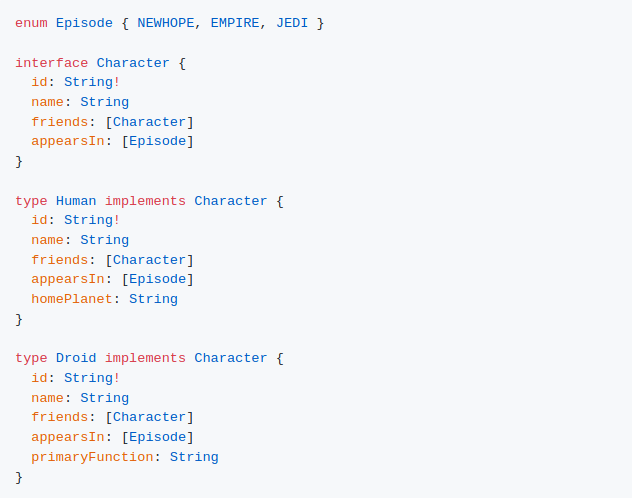
\includegraphics[width=0.7\textwidth]{schema.png}
  \end{center}
\end{frame}

\begin{frame}{REST vs GraphQL}
  \begin{center}
   \begin{columns}
     \begin{column}{0.5\textwidth}
    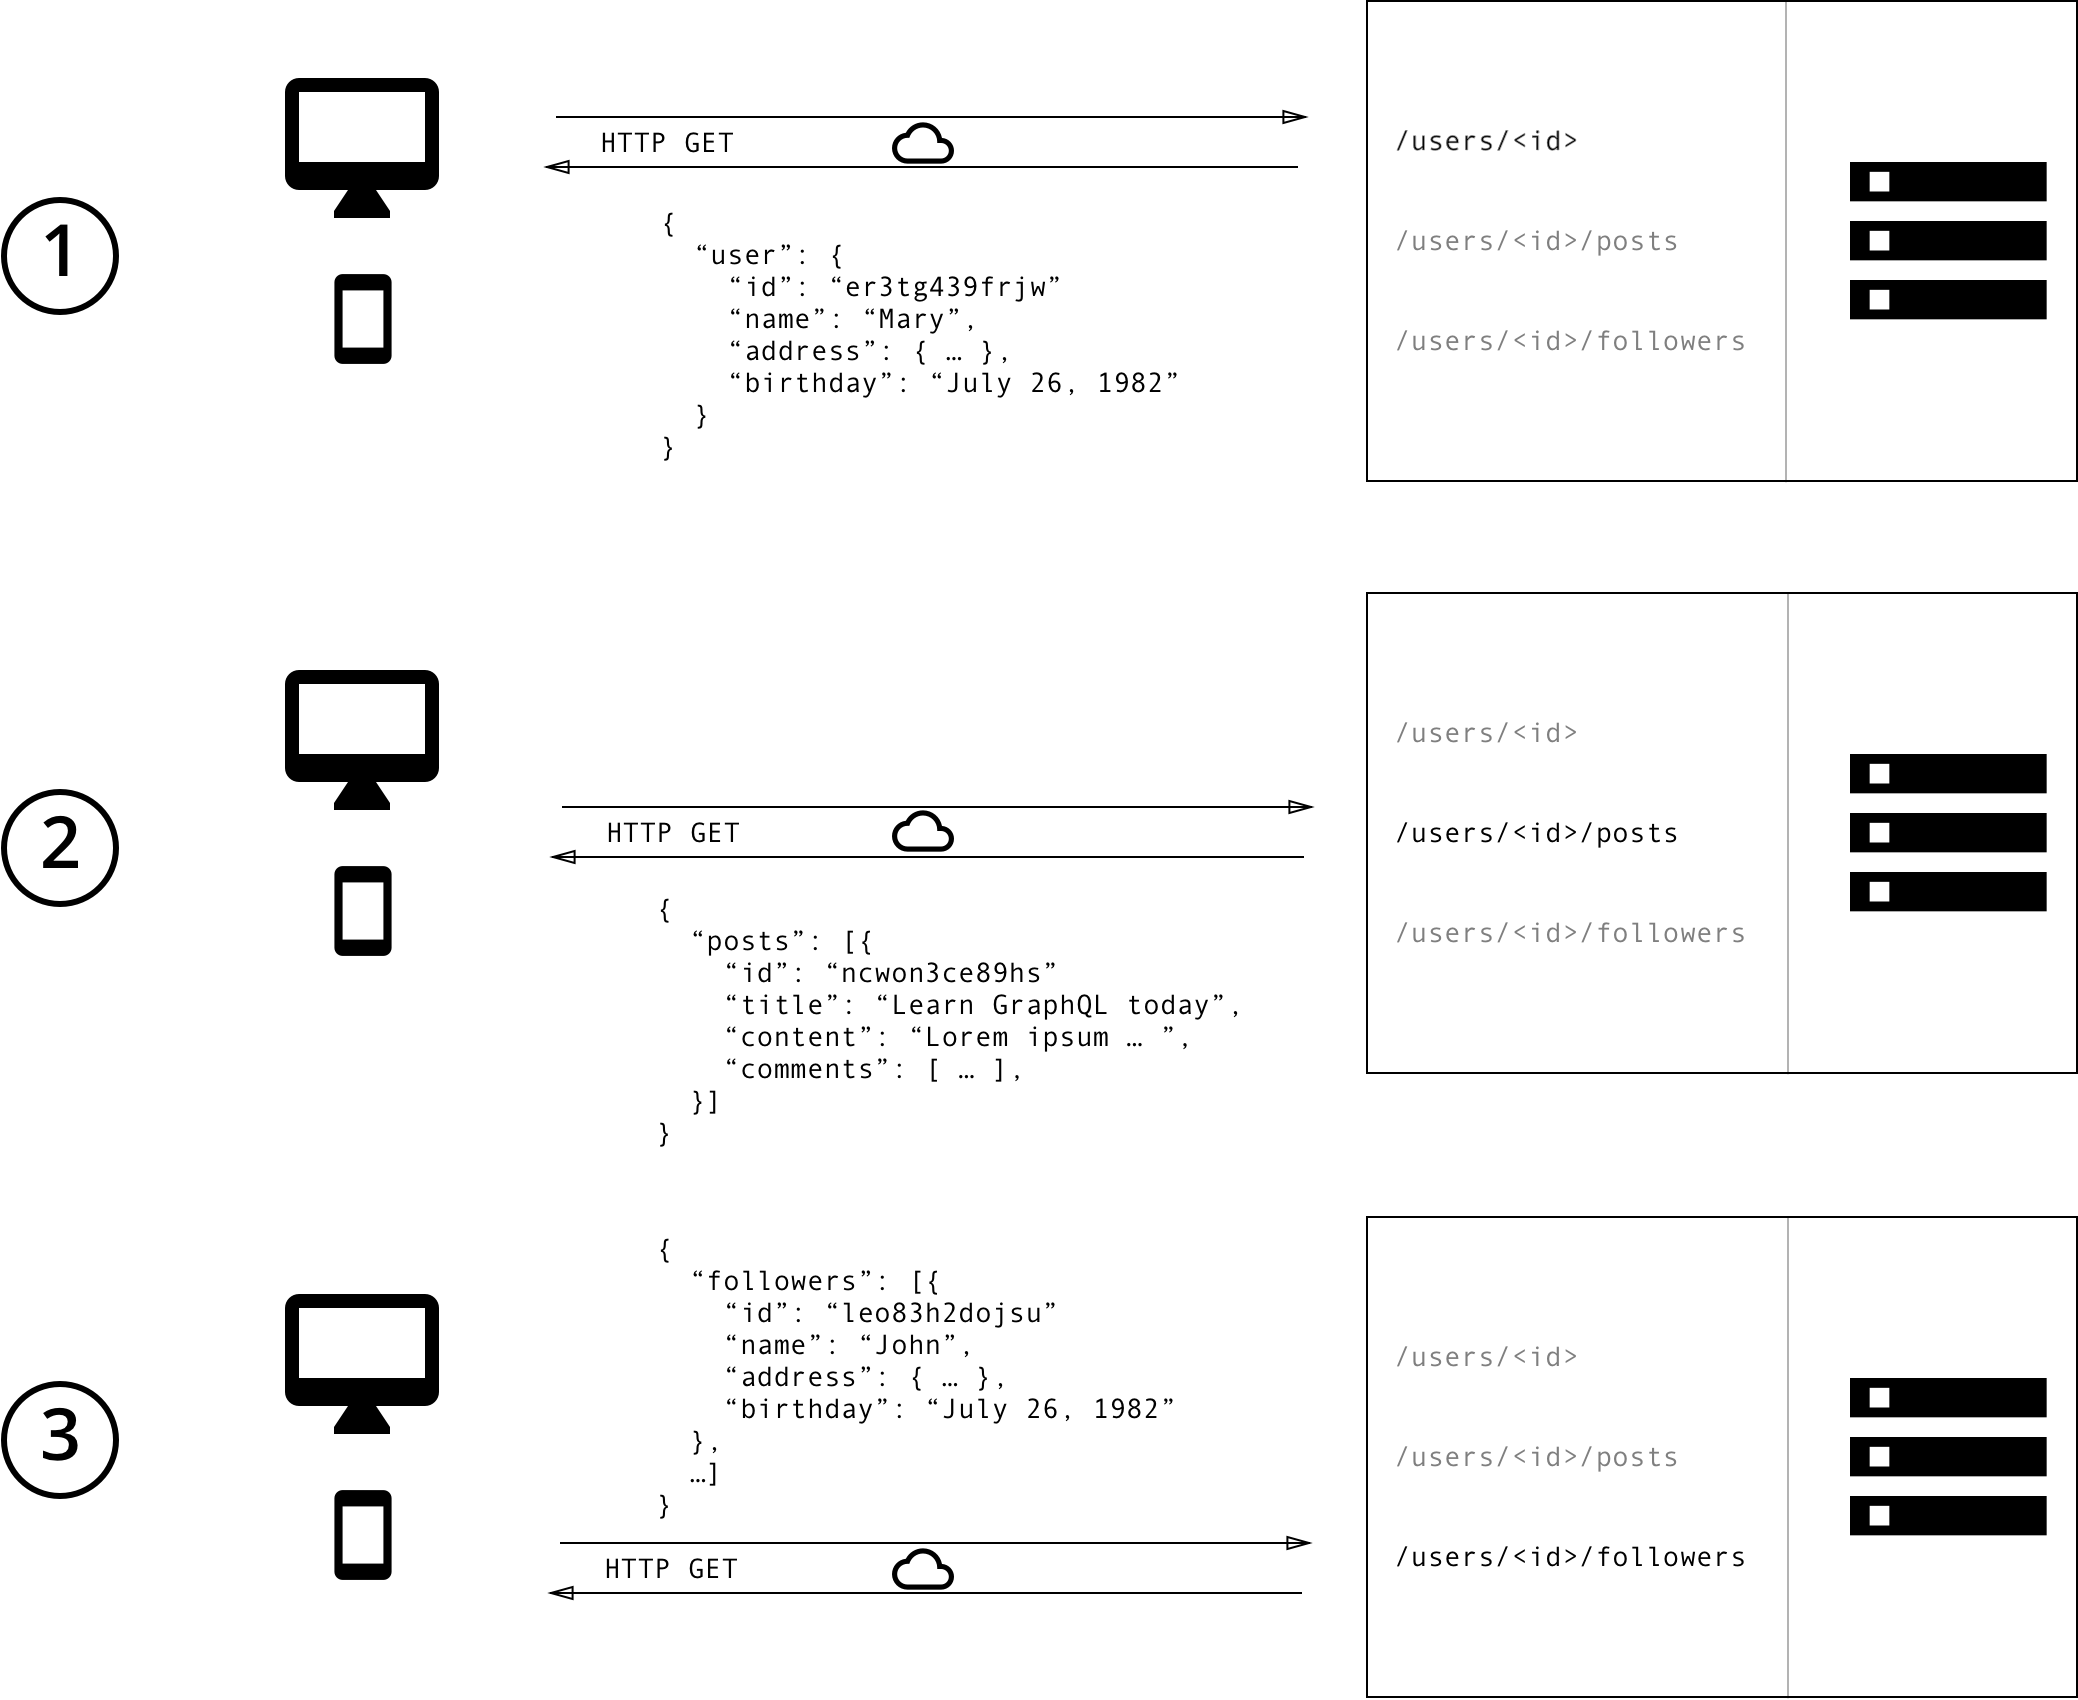
\includegraphics[width=0.9\textwidth]{REST.png}
     \end{column}
     \begin{column}{0.5\textwidth}  %%<--- here
    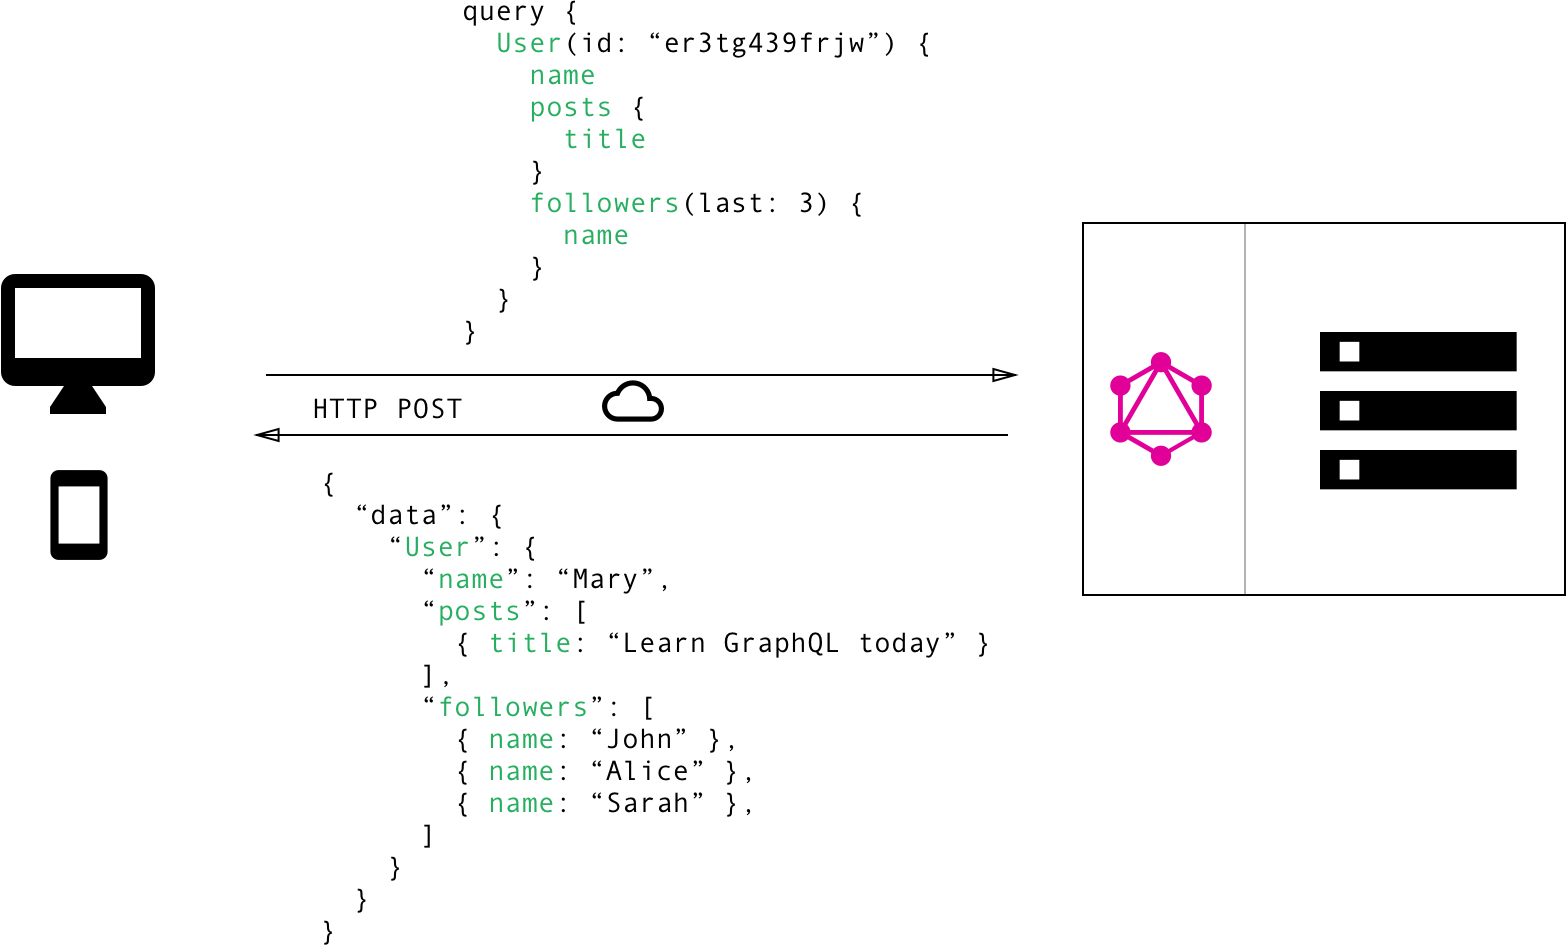
\includegraphics[width=0.9\textwidth]{howgraphql.png}
     \end{column}
     \end{columns}
  \end{center}
\end{frame}


\section{Python}
\begin{frame}
  \begin{center}
    
\includegraphics[width=0.7\textwidth]{graphenepython.png}
  \end{center}
\end{frame}
\section{}
\begin{frame}
  \centering
  \Huge{¿Preguntas?}
  
\includegraphics[width=0.7\textwidth]{preguntas.png}
\end{frame}

\begin{frame}{References}
    \centering
      \begin{itemize}
          \item \WebLink{https://graphql.org/}{GraphQL Official Page (graphql.org)} 
          \item \WebLink{https://www.howtographql.com/}{The Fullstack tutorial for GraphQL (howtographql.com)}
          \item \WebLink{https://graphene-python.org/}{Graphene-Python (graphene-python.com)}
          \item \WebLink{https://docs.graphene-python.org/projects/django/en/latest/}{Graphene-Django (https://docs.graphene-python.org/projects/django/en/latest/)}
      \end{itemize}
\end{frame}

\begin{frame}
    \centering
      \begin{itemize}
        \item Alejandro Almira
        \item alejandroalmira [at] protonmail.com
        \item aalmiramolla [at] linkedin github gitlab telegram
      \end{itemize}
\end{frame}

\end{document}

%%% Local Variables:
%%% mode: latex
%%% TeX-master: t
%%% End:
